\documentclass[journal,article,submit,pdftex]{Definitions/mdpi}

\usepackage{tabularx}
\usepackage{caption}

\firstpage{1}
\setlength{\headheight}{20.0pt}
\makeatletter
\setcounter{page}{\@firstpage}
\makeatother

\pubvolume{1}
\issuenum{1}
\articlenumber{0}
\pubyear{2025}
\copyrightyear{2025}

\datereceived{}
\daterevised{} % Comment out if no revised date
\dateaccepted{}
\datepublished{}

\hreflink{https://www.mdpi.com/journal/iot} % If needed, change journal link

\Title{Implementation of a physics laboratory for engineering through IoT-based retrofitting in a hybrid learning environment.}

\Author{Walter Santiago Sosa Mej\'ia}
\AuthorNames{Walter Santiago Sosa Mej\'ia}
\AuthorCitation{Sosa Mej\'ia, W.S.}

\address{%
\quad Pontificia Universidad Cat\'olica del Ecuador, Sede Esmeraldas; wssosa@pucese.edu.ec}

%-------------------------------------------------
% ABSTRACT
%-------------------------------------------------

\abstract{Updating physics laboratories in institutions with limited budgets often involves a practical tension: expanding access while preserving equipment that is still functional. This work designs and validates a remote laboratory for the study of Uniformly Accelerated Rectilinear Motion (MRUA) using an IoT \textit{retrofitting} strategy over existing infrastructure. The solution integrates an ESP32 (control module), infrared passage sensors, and a web interface for real-time operation and monitoring. Validation was conducted through 70 independent trials (35 remote and 35 in-person), comparing detection times and derived kinematic magnitudes between both modalities. Results show that the remote system reproduces the behavior of the reference setup with bounded differences and stable operation throughout the experimental campaign. Overall, the findings support IoT \textit{retrofitting} as a technically viable and scalable alternative to strengthen experimental teaching in hybrid scenarios without requiring full laboratory replacement.}

\keyword{Retrofitting; Internet of Things; Remote laboratories; MRUA; Low-cost instrumentation; Cloud services; Engineering education}

\begin{document}

%-------------------------------------------------
% INTRODUCTION
%-------------------------------------------------

\section{Introduction}

Physics laboratories remain the space where theoretical models are contrasted with measurable evidence, and therefore they retain a central role in engineering education. However, many of these environments were designed for strictly in-person operation: local instrumentation, manual recording, and limited data traceability. In parallel, the digitalization of scientific infrastructure and cyber-physical architectures has opened the possibility of operating real experiments remotely, with online supervision and data capture \cite{r1}. The experience accumulated after the COVID-19 pandemic made this need more visible and accelerated the adoption of cloud-connected laboratories \cite{r2}.

In Latin America, this transition often faces a concrete limitation: laboratories operate with equipment that is still useful but was not conceived for automation or remote access. The case of the Pontificia Universidad Cat\'olica del Ecuador, Esmeraldas campus, reflects this reality: there are functional setups for kinematics (track and low-friction cart), but without a digital layer that allows remote control, recording, and sharing of the experiment. In this context, low-cost IoT \textit{retrofitting} is not proposed as a full replacement of the laboratory, but as a progressive and viable modernization strategy \cite{r3,r4}.

\subsection{Related Work and Research Gap}

Recent literature shows significant advances in the modernization of physics laboratories through digital technologies, particularly via remote and hybrid laboratories and IoT-based \textit{retrofitting} strategies. Studies such as Lahme \textit{et al.} \cite{r1} document increased use of microcontrollers, sensors, and digital platforms in laboratory courses, highlighting both their potential and technical adoption barriers. Complementarily, work focused on remote control of physical systems, such as Guerrero-Osuna \textit{et al.} \cite{r4} and Fuertes \textit{et al.} \cite{r3}, demonstrates the feasibility of integrating embedded hardware, cloud services, and web interfaces to operate real experiments with adequate response times.

In the specific context of \textit{retrofitting} existing equipment, Viswanadh \textit{et al.} \cite{r2} propose low-cost architectures that instrument pre-existing laboratory setups without structural modifications, while Lustig \textit{et al.} \cite{r5} introduce modular platforms that decouple experimental hardware from access and visualization services. Zhao \cite{r6}, in turn, extensively reviews solutions based on mass-market sensors and video analysis, showing that it is possible to obtain reasonably high-quality measurements using accessible and widely available devices.

However, despite these contributions, several limitations are evident in current literature. First, many studies focus on functional demonstrations of remote platforms or usability evaluations, without deep quantitative validation of experimental fidelity against in-person reference setups. Second, there is a lack of studies that systematically analyze the technical performance of classic physics experiments such as kinematics when executed remotely, considering metrics such as detection-time error, internal data coherence, and system stability. Finally, few studies address these issues in resource-constrained contexts, where reusing existing equipment through \textit{retrofitting} is especially relevant.

Within this context, this work differs by proposing and validating a hybrid physics laboratory model based on IoT \textit{retrofitting}. To contextualize our contribution within modern IoT architectures, we adopt the layered approach proposed by Dizdarevic and Jukan \cite{r7}, who highlight the importance of integrating edge and cloud computing capabilities to reduce latency in educational environments; we apply this lesson by using the control device for edge-side processing. Likewise, to ensure operational continuity and universal accessibility, we follow Azad's principles \cite{r8} for deploying IoT-based remote laboratories, ensuring robustness against disconnections. Finally, our system validation aligns with the digital-twin methodology described by Palmer \textit{et al.} \cite{r9}, using direct comparison between physical sensor data (the "real twin") and the expected theoretical model to ensure rigorous quantitative verification.

%-------------------------------------------------
% MATERIALS AND METHODS
%-------------------------------------------------

\section{Materials and Methods}
\label{sec:metodos}

\subsection{Research Design}

This research was designed as an applied technical study focused on the design, construction, and validation of a remotely operated physics laboratory prototype based on IoT technologies. A quantitative descriptive approach was adopted because the core analysis variables are measurable physical quantities (detection times, registered events, and failures) obtained from system instrumentation logs and compared across operating modalities without intervention on human participant groups. The methodological approach follows the logic of \textit{Design Science Research} (DSR), in which the central objective is to build and systematically evaluate a technological artifact \cite{r11}. As an organizational reference, ISO/IEC~15288 system life-cycle processes were considered to structure requirements, design, implementation, integration, and operation phases \cite{r12}.

Within this scope, the study is restricted to technical evaluation of the Uniformly Accelerated Rectilinear Motion (MRUA) experiment, specifically the accuracy and consistency of physical variables measured and calculated by the remote system compared with an equivalent in-person reference setup.

%-------------------------------------------------
\subsection{Hardware and Software Used}

To ensure clear and reproducible presentation, the materials are grouped into two tables: hardware components (Table~\ref{tab:hardware}) and software tools (Table~\ref{tab:software}). Figure~\ref{fig:arquitectura} summarizes how these elements are integrated in the overall system architecture.

\begin{table}[H]
	\caption{Hardware components of the IoT-based hybrid physics laboratory prototype.\label{tab:hardware}}
	\small
	\begin{adjustwidth}{-\extralength}{0cm}
		\renewcommand{\arraystretch}{1.5}
		\renewcommand{\tabularxcolumn}[1]{m{#1}}
		\begin{tabularx}{\fulllength}{>{\raggedright\arraybackslash}m{4.5cm}Xc}
			\toprule
			\textbf{Device Category} & \textbf{Consolidated Technical Specification} & \textbf{References} \\
			\midrule
			Mechanical experimental system & Hot Wheels\textsuperscript{\textregistered} track used as straight-motion rail and low-friction cart adapted for kinematics practice & \cite{r13, r14} \\
			Sensing and data acquisition system & Four infrared sensors for passage detection and time measurement & \cite{r15} \\
			IoT control and processing unit & DevKit control module (30 pins, USB-C, integrated WiFi and Bluetooth connectivity) & \cite{r16} \\
			Mechanical structure and physical support & 3D-printed supports, reinforcements, and mechanical assemblies for mounting sensors, actuators, and structural elements & \cite{r17, r18, r19, r20} \\
			Actuators and motion control & SG90 servo motor (180\textdegree), bipolar NEMA 17 stepper motor, and L298N H-bridge module for motion control & \cite{r21, r22, r23} \\
			Local user interface & 20x4 LCD display with I\textsuperscript{2}C interface and mechanical pushbutton for local interaction & \cite{r24, r25} \\
			Communication and connectivity & IEEE 802.11 wireless standard (WiFi), USB Type-C cable, and Dupont wires for electrical interconnection & \cite{r26, r27, r28} \\
			Power and protection system & 12 V / 1 A AC--DC adapter and plastic project enclosure (135 $\times$ 75 $\times$ 40 mm) & \cite{r29, r30} \\
			Remote visualization system & Insta360 Link webcam with 4K resolution and AI-assisted tracking functions & \cite{r31} \\
			IoT server and system management & Raspberry Pi 4 Model B for communication management, storage, and system monitoring & \cite{r32} \\
			\bottomrule
		\end{tabularx}
	\end{adjustwidth}
\end{table}


\begin{table}[H]
	\caption{Software tools used in the IoT-based hybrid physics laboratory system.\label{tab:software}}
	\small
	\begin{adjustwidth}{-\extralength}{0cm}
		\renewcommand{\arraystretch}{1.5}
		\renewcommand{\tabularxcolumn}[1]{m{#1}}
		\begin{tabularx}{\fulllength}{>{\raggedright\arraybackslash}m{3.5cm}X>{\centering\arraybackslash}m{3.5cm}c}
			\toprule
			\textbf{System Layer} & \textbf{Software Tools} & \textbf{Versions} & \textbf{References} \\
			\midrule
			IoT communication & EMQX, MQTTX Desktop & 5.10.2; 1.12.1 & \cite{r33, r34} \\
			Backend and services & Node.js (LTS), Express & 24.11.1; 5.1.0 & \cite{r35, r36} \\
			Data persistence & MongoDB Server, MongoDB Driver, Mongoose & 8.2.2; 6.3.0; 8.5.1 & \cite{r37, r38} \\
			Frontend and visualization & Next.js, React & 16.0; 19.2.0 & \cite{r39, r40} \\
			Embedded development & Arduino IDE & 2.3.4 & \cite{r41} \\
			Languages and support & Python & 3.14.1 & \cite{r42} \\
			\bottomrule
		\end{tabularx}
	\end{adjustwidth}
\end{table}

\subsection{Overall System Architecture}

The overall system architecture is organized into three clearly differentiated layers \cite{r10} (Figure~\ref{fig:arquitectura}). Layer~1 groups experiment perception elements, including the MRUA cart, the track, four infrared sensors, the experiment camera, and the control module, which acquires sensor signals and sends them via MQTT over WiFi. Layer~2 corresponds to local network and server infrastructure, formed by the WiFi router/access point and Raspberry~Pi, where the EMQX broker, video server, and web API run to process data. Finally, Layer~3 includes the web-based user interface from which instructors and students can visualize data tables and position/velocity/acceleration plots, watch experiment video, and send control commands.

\begin{figure}[H]
\centering
\includegraphics[width=\textwidth]{figures/fig1_arquitectura_labfisica.png}
\caption{Three-layer architecture of the physics laboratory with IoT \textit{retrofitting}. Diagram built following the fundamental three-layer model \cite{r10} using Eraser~\cite{r43}.}
\label{fig:arquitectura}
\end{figure}

\begin{figure}[H]
\centering
\includegraphics[width=0.8\textwidth]{figures/Hardware connection diagram of the proposed prototype.png}
\caption{Control-module diagram. Image generated with ChatGPT assistance \cite{r44}.}
\label{fig:hardware_connection}
\end{figure}

\begin{table}[H]
	\caption{Detailed system connections and control-module pin assignment.\label{tab:connections}}
	\small
	\begin{adjustwidth}{-\extralength}{0cm}
		\renewcommand{\arraystretch}{1.3}
		\renewcommand{\tabularxcolumn}[1]{m{#1}}
		\begin{tabularx}{\fulllength}{clXccc}
			\toprule
			\textbf{No.} & \textbf{Component} & \textbf{Function in Experiment} & \textbf{Control Pin} & \textbf{Signal Type} & \textbf{Power} \\
			\midrule
			1  & Sensor S1      & Motion-start detection                    & GPIO 15 & Digital input (PULLUP) & 5 V / GND    \\
			2  & Sensor S2      & Intermediate section 1 detection          & GPIO 25 & Digital input (PULLUP) & 5 V / GND    \\
			3  & Sensor S3      & Intermediate section 2 detection          & GPIO 12 & Digital input (PULLUP) & 5 V / GND    \\
			4  & Sensor S4      & End-of-track detection                    & GPIO 13 & Digital input (PULLUP) & 5 V / GND    \\
			5  & Manual button  & Experiment start/cancel                   & GPIO 18 & Digital input (PULLUP) & GND          \\
			6  & Servo motor    & Initial cart push/release                 & GPIO 5  & PWM                    & 5 V / GND    \\
			7  & L298N -- ENA   & Motor acceleration control (NRUA)         & GPIO 14 & PWM                    & 5 V / GND    \\
			8  & L298N -- IN1   & DC motor direction                        & GPIO 27 & Digital output         & ---          \\
			9  & L298N -- IN2   & DC motor direction                        & GPIO 26 & Digital output         & ---          \\
			10 & LCD 16$\times$2 -- SDA & I2C communication (data)         & GPIO 21 & I2C                    & 5 V / GND    \\
			11 & LCD 16$\times$2 -- SCL & I2C communication (clock)        & GPIO 22 & I2C                    & 5 V / GND    \\
			12 & DC motor       & Accelerated-motion generation             & L298N   & Power                  & 11--12 V     \\
			13 & Common ground  & System electrical reference               & GND     & ---                    & Common       \\
			\bottomrule
		\end{tabularx}
	\end{adjustwidth}
\end{table}

\subsection{Population, Sample, and Experimental Environment}

This study does not involve a population of human subjects or organizational units; instead, it evaluates an instrumented physical system from a technical perspective. Therefore, rather than defining population and sample in the classical quantitative-research sense, this subsection describes the laboratory environment and trial planning. A total of 70 trials were carried out: 35 in-person and 35 remote.

The experiment was conducted in the physics laboratory of the Pontificia Universidad Cat\'olica del Ecuador, Esmeraldas campus, which has a leveled workbench, regulated power access, and local network connectivity through a WiFi access point. The Hot Wheels\textsuperscript{\textregistered} track \cite{r13}, low-friction cart \cite{r14}, four infrared sensors \cite{r15}, control module \cite{r16}, and Insta360 Link camera \cite{r31} were installed there to form the physical MRUA setup. The Raspberry~Pi~4 used as IoT server \cite{r32} was located in the same laboratory and connected to both the WiFi access point \cite{r27} and the institutional wired network.

%-------------------------------------------------
\subsection{Implementation Procedure}

The procedure used to develop and evaluate the prototype was organized into four stages aligned with the study objectives: (i) system design and IoT architecture definition, (ii) hardware/software implementation, (iii) experimental setup and trial execution in remote and in-person modes, and (iv) technical validation.

First, requirements were gathered with the course instructor responsible for Physics, considered an MRUA subject-matter expert. This stage identified events the system had to register (cart passing each sensor), minimum information needed to describe the experiment, and acceptable setup conditions. From these inputs, the remote-laboratory IoT architecture was defined, specifying hardware components, software services, and data flow among ESP32, MQTT server, backend, and web app. Design decisions were documented in \texttt{README} files of the public \textit{RemotePhysicsLab} repository \cite{r45}, in the \texttt{frontend} and \texttt{backend} folders.

In the second stage, the IoT prototype was implemented (Figure~\ref{fig:arquitectura}). The physical track was built and infrared sensors were installed at fixed positions along the cart path. The control module was programmed in Arduino IDE to read sensor states and send timestamped MQTT messages to the MQTT server running on Raspberry~Pi. In parallel, the experiment camera and video server were configured so the stream could be consumed from a web browser. Unit tests were performed to verify correct sensor reading, WiFi connectivity, publication on defined MQTT topics, and continuous video reception.

Next, the experimental environment was configured and trials were executed. Cart starting point, track inclination, and sensor positions were fixed and kept constant across tests. Trial series were conducted in two modalities: remote operation through the web interface (user triggers experiment, observes movement through near-real-time video, and detection times are automatically recorded) and in-person operation using a reference setup without IoT as baseline. In both modalities, the experiment was repeated multiple times to obtain sufficient records.

Finally, technical validation was performed. Data from remote and in-person setups were collected and organized in comparative tables by sensor and repetition. Agreement of detection times between modalities was evaluated, verification was made that the remote system registered all expected events, and qualitative incidents related to system stability (service drops, disconnections, restart needs) were documented.

\begin{figure}[H]
\centering
\includegraphics[width=\textwidth]{figures/Experimental procedure flowchart.png}
\caption{Data flow during laboratory operation.
Infrared sensor readings associated with cart passage are sent by the control module to the MQTT server.
The backend processes messages, stores them in MongoDB, and exposes them to the web application, which presents data and experiment video to the user. Figure created with the AI-assisted diagramming tool Eraser \cite{r43}.}
\label{fig:flujo-datos}
\end{figure}

%-------------------------------------------------
\subsection{Evaluation Metrics}

Technical validation focuses on quantifying association and agreement between measurements obtained in in-person modality and those registered by the IoT system. The objective is to determine whether IoT-based \textit{retrofitting} can replicate the stability and precision of the traditional setup. The experimental campaign included 70 total trials, divided into 35 manual (in-person) and 35 automated (remote) records.

As the main performance metric, Pearson's correlation coefficient (\(r\)) is used to evaluate how faithfully the remote laboratory reproduces behavior observed in the reference physical setup. The coefficient is calculated independently for each of the four sensors (S1 to S4). Since trials in both modalities were independent physical events, the analysis does not seek strict trial-by-trial correspondence; instead, it verifies that both systems capture MRUA dynamics consistently.

The coefficient is defined as:

\begin{equation}
r = \frac{\sum_{i=1}^{n} (x_i - \bar{x})(y_i - \bar{y})}{\sqrt{\sum_{i=1}^{n} (x_i - \bar{x})^2} \sqrt{\sum_{i=1}^{n} (y_i - \bar{y})^2}}
\label{eq:pearson}
\end{equation}

where \(x_i\) represents in-person measured times and \(y_i\) remote measured times for \(n=35\) trials per modality, with means \(\bar{x}\) and \(\bar{y}\). A value of \(r\) close to 1 supports that IoT instrumentation captures natural kinematic variability with fidelity comparable to in-person timing.



%-------------------------------------------------

\subsection{Data Analysis Methods}

Data recorded by the IoT prototype (hybrid modality) and by the in-person reference setup were exported as structured text files containing timestamps associated with cart passage through each sensor and trial configuration. These records were organized in spreadsheets and then processed with scripts developed in Python~3.14.1 \cite{r42}.

The analysis focused on consistency of sensor passage times and computation of Pearson correlation between hybrid and in-person modalities. Scatter plots and histograms were generated to visualize proximity between measurements and detect possible prototype deviations. Numerical and graphical results are presented in the Results section.

In a first stage, data from both modalities were integrated into comparative tables that grouped, by trial, passage times recorded by the hybrid system and by the in-person setup. In a second stage, scatter plots and histograms were generated to visualize agreement and validate prototype consistency through correlation analysis.


%-------------------------------------------------
\subsection{Validity and Reliability Control}

Validity and reliability control focused on ensuring that measurements made by the IoT prototype were coherent with expected MRUA physical behavior and comparable with those obtained in the in-person reference setup.

First, measurement validity was verified by specific cart-detection tests using infrared sensors. Controlled test runs were executed while monitoring control-module digital inputs and MQTT-published messages in real time. Sensor height and orientation were adjusted until clean active/inactive transitions were achieved without spurious triggering due to ambient noise or undesired reflections. The track has an effective length of 160~cm, with four sensors distributed at 53.2~cm intervals, providing well-defined distances for speed and acceleration calculations from passage times.

Additionally, fixed distances between sensors were carefully measured with a conventional measuring tape of adequate resolution, so derived kinematic calculations (average speed and acceleration) were based on consistent reference values. The in-person setup was used as baseline for contrasting times and derived magnitudes obtained with the IoT prototype.

For reliability and repeatability, 70 repeated trials were carried out (35 in-person and 35 remote) under identical setup conditions (same track inclination, same cart initial position, same sensor locations). Variability of passage times and estimated accelerations was analyzed through basic descriptive statistics (mean and standard deviation) as indicators of measurement stability. Records with obvious anomalies (detection failures, communication interruptions, or evident launch errors) were explicitly discarded from comparative analysis and documented as atypical events to avoid biasing conclusions.

To reduce internal-validity threats, experiments were performed under controlled conditions: track and sensors remained fixed on the same workbench, setup manipulation between trial series was avoided, and stable lighting was maintained to prevent relevant variations in sensor response and video quality. The control module locally recorded timestamps for each detection event so network latency affected only remote visualization and not physical-data timestamping.

Regarding external validity, this study is limited to technical evaluation of a hybrid-laboratory prototype for one specific dynamics experiment (MRUA) in one specific setting (PUCE Esmeraldas physics laboratory). The goal is not to generalize to learning indicators or usability perceptions, but to demonstrate that a \textit{retrofitting} and IoT architecture can reproduce reference in-person measurements with sufficient precision and stability under controlled conditions.

%-------------------------------------------------

\subsection{Reproducibility and Ethics}

To facilitate reproducibility, the source code of the hybrid-laboratory prototype and configuration files required to deploy backend, MQTT server, and web application were published in a public GitHub repository \cite{r45}. The \texttt{README.md} documents steps to clone the repository, install dependencies, configure environment variables, and run involved services, together with recommended hardware/software versions. This allows other teams to replicate the proposed architecture with a similar combination of control module, Raspberry~Pi, EMQX, and web application, or adapt the design to their own physics laboratories.

Regarding ethical and institutional considerations, prototype development and evaluation were conducted with explicit authorization from the Pontificia Universidad Cat\'olica del Ecuador, Esmeraldas campus, both for use of the physics laboratory and institutional mention in the manuscript. The study did not involve personal-data collection nor students as research subjects; therefore, additional individual consent protocols were not required. Activities were limited to responsible use of laboratory infrastructure and recording physical variables associated with the MRUA experiment.

%-------------------------------------------------
% RESULTS
%-------------------------------------------------

\section{Results}

This section presents results from the experimental validation of the proposed IoT-based \textit{retrofitting} system. The analysis focuses on data-capture stability and statistical correlation between remote (IoT) and in-person (traditional) modalities. The dataset comprises \(N=70\) independent trials (35 remote and 35 in-person).

\subsection{Experimental Setup and Prototype Implementation}

The physical implementation of the prototype integrates the mechanical structure, the electronic sensing layer, and the IoT control unit. Because of the track length (160 cm), the setup is shown in detailed sections to visualize component distribution. Figure~\ref{fig:montaje_detalles} presents the four main route sections: (a) start, (b) section 2, (c) section 3, and (d) arrival point. A general view of the complete prototype is shown in Figure~\ref{fig:vista_general}. The detection system consists of four infrared sensors distributed at precise 53.2 cm intervals along the structure to capture total time from automated cart release to the end of the track.
\begin{figure}[H]
\centering
\subfloat[]{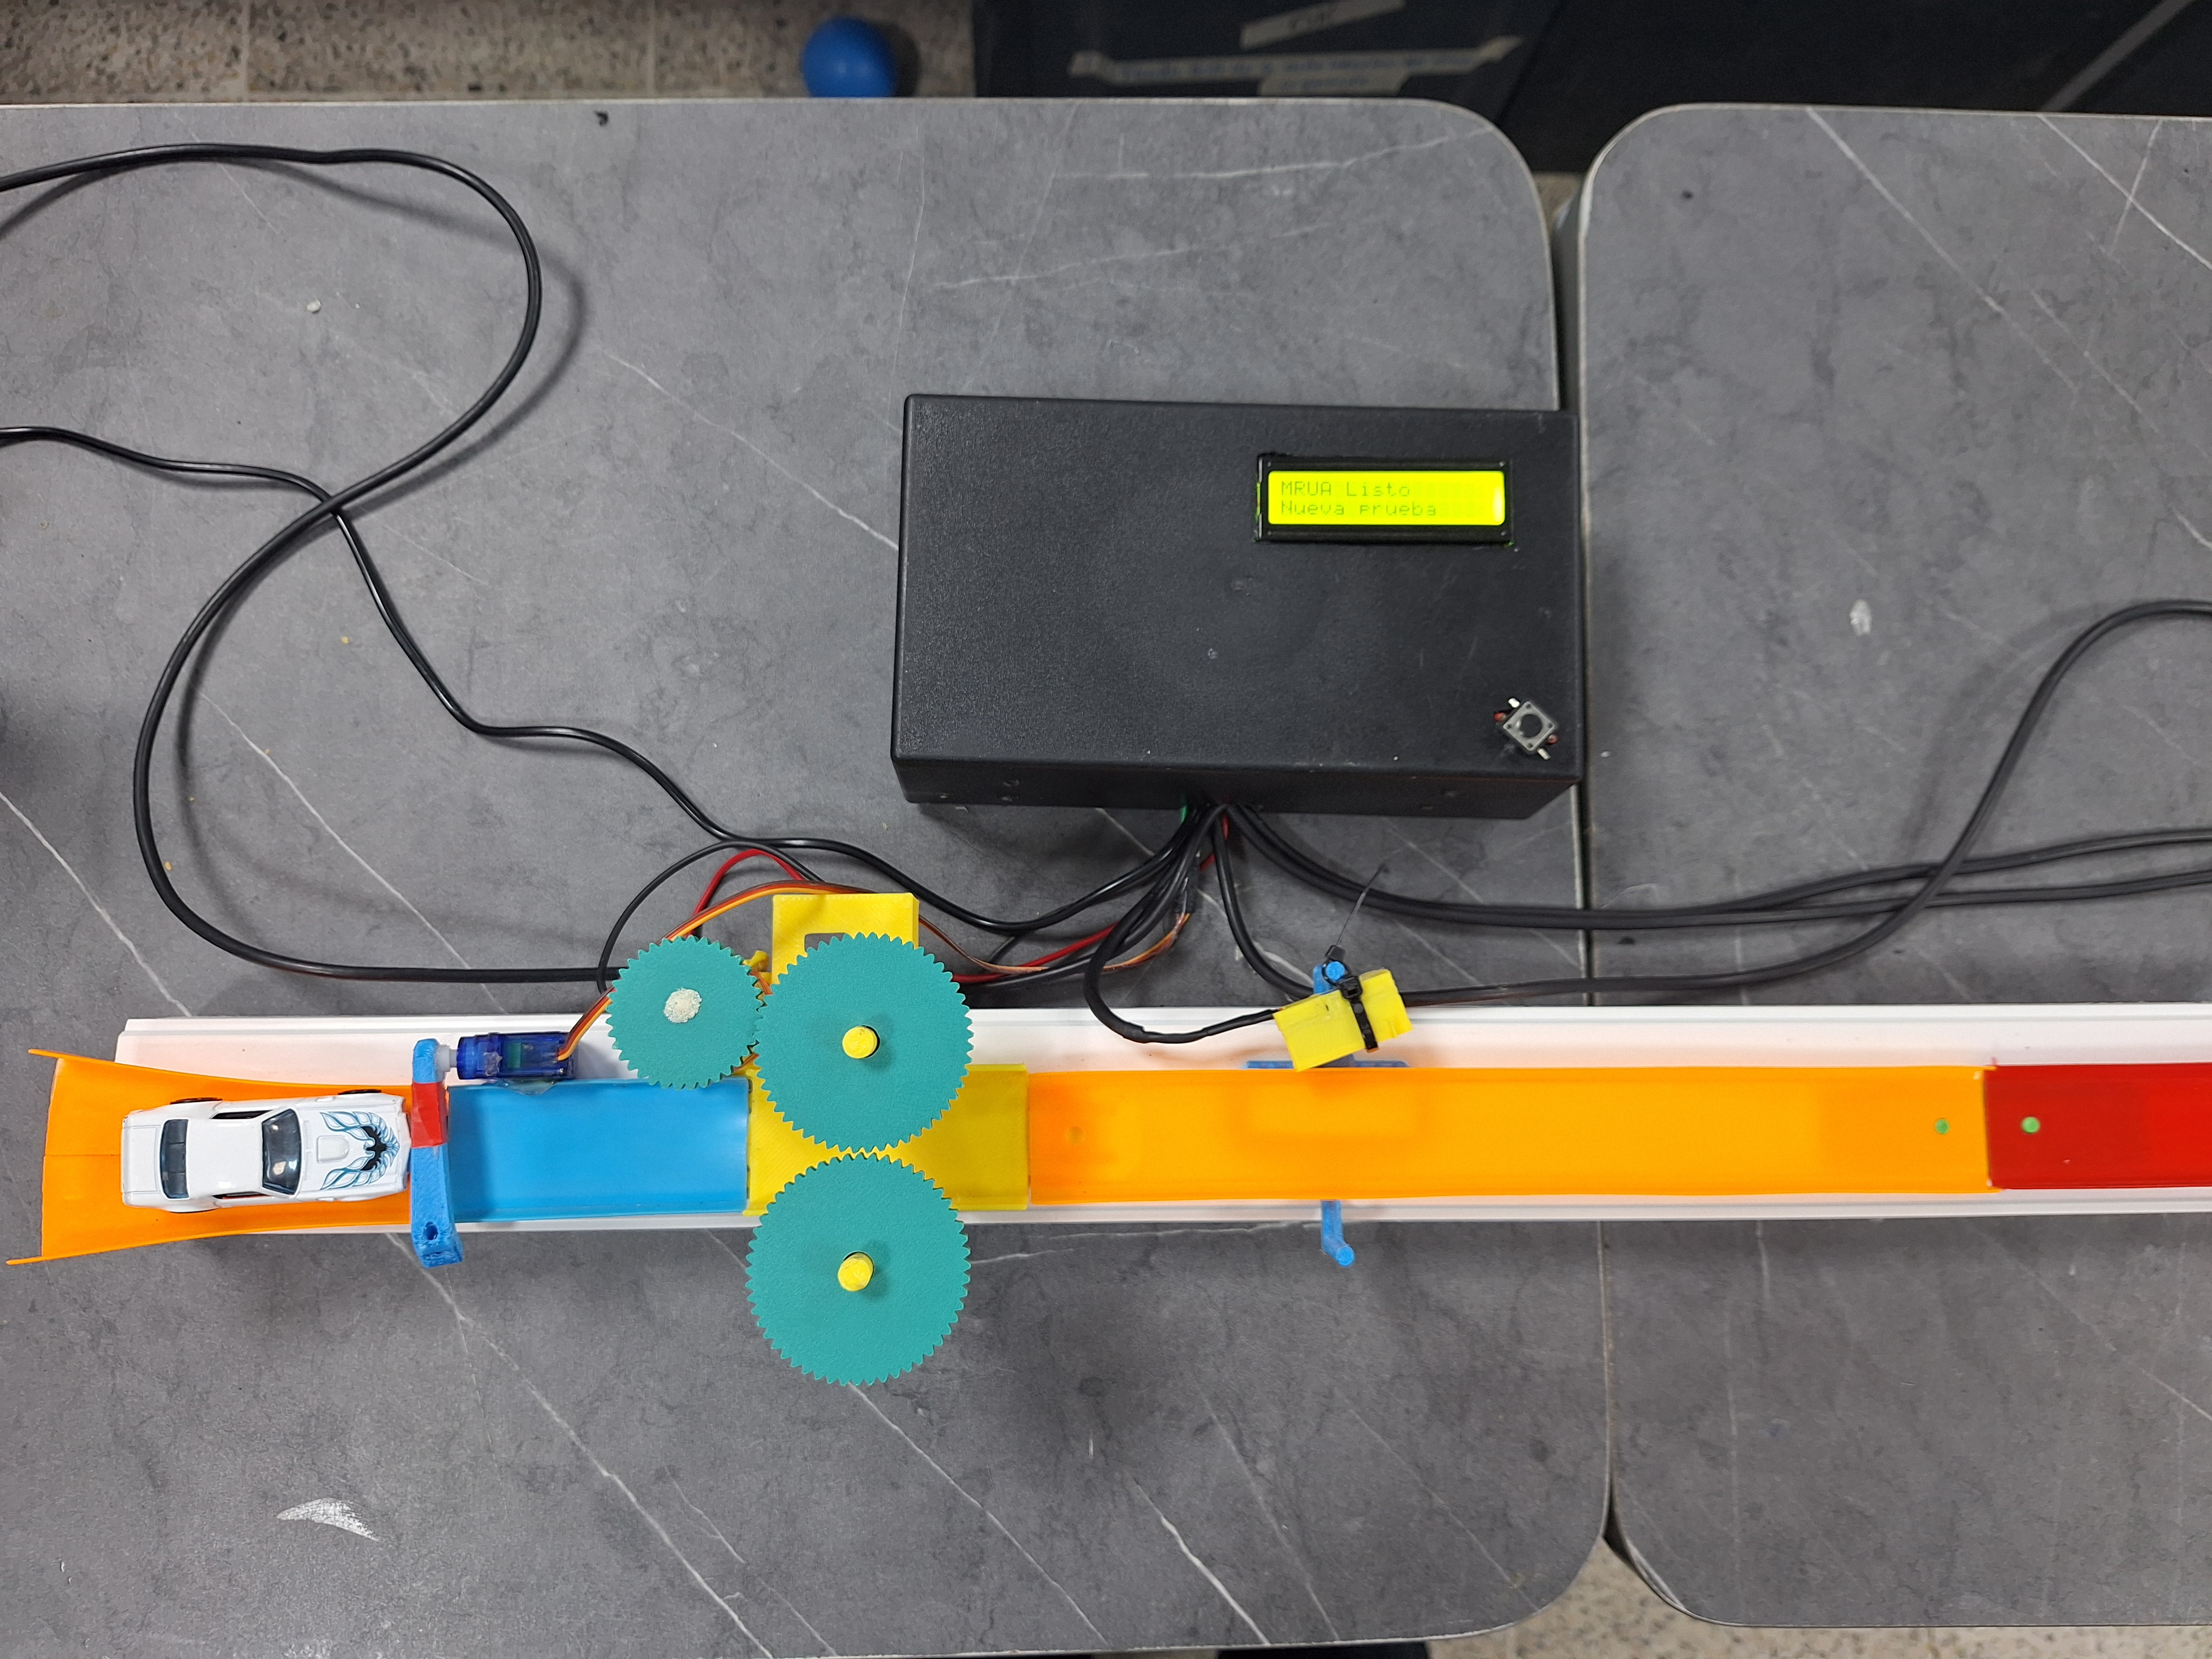
\includegraphics[width=0.45\textwidth]{figures/setup_overview_inicio.jpg}}
\hspace{0.5cm}
\subfloat[]{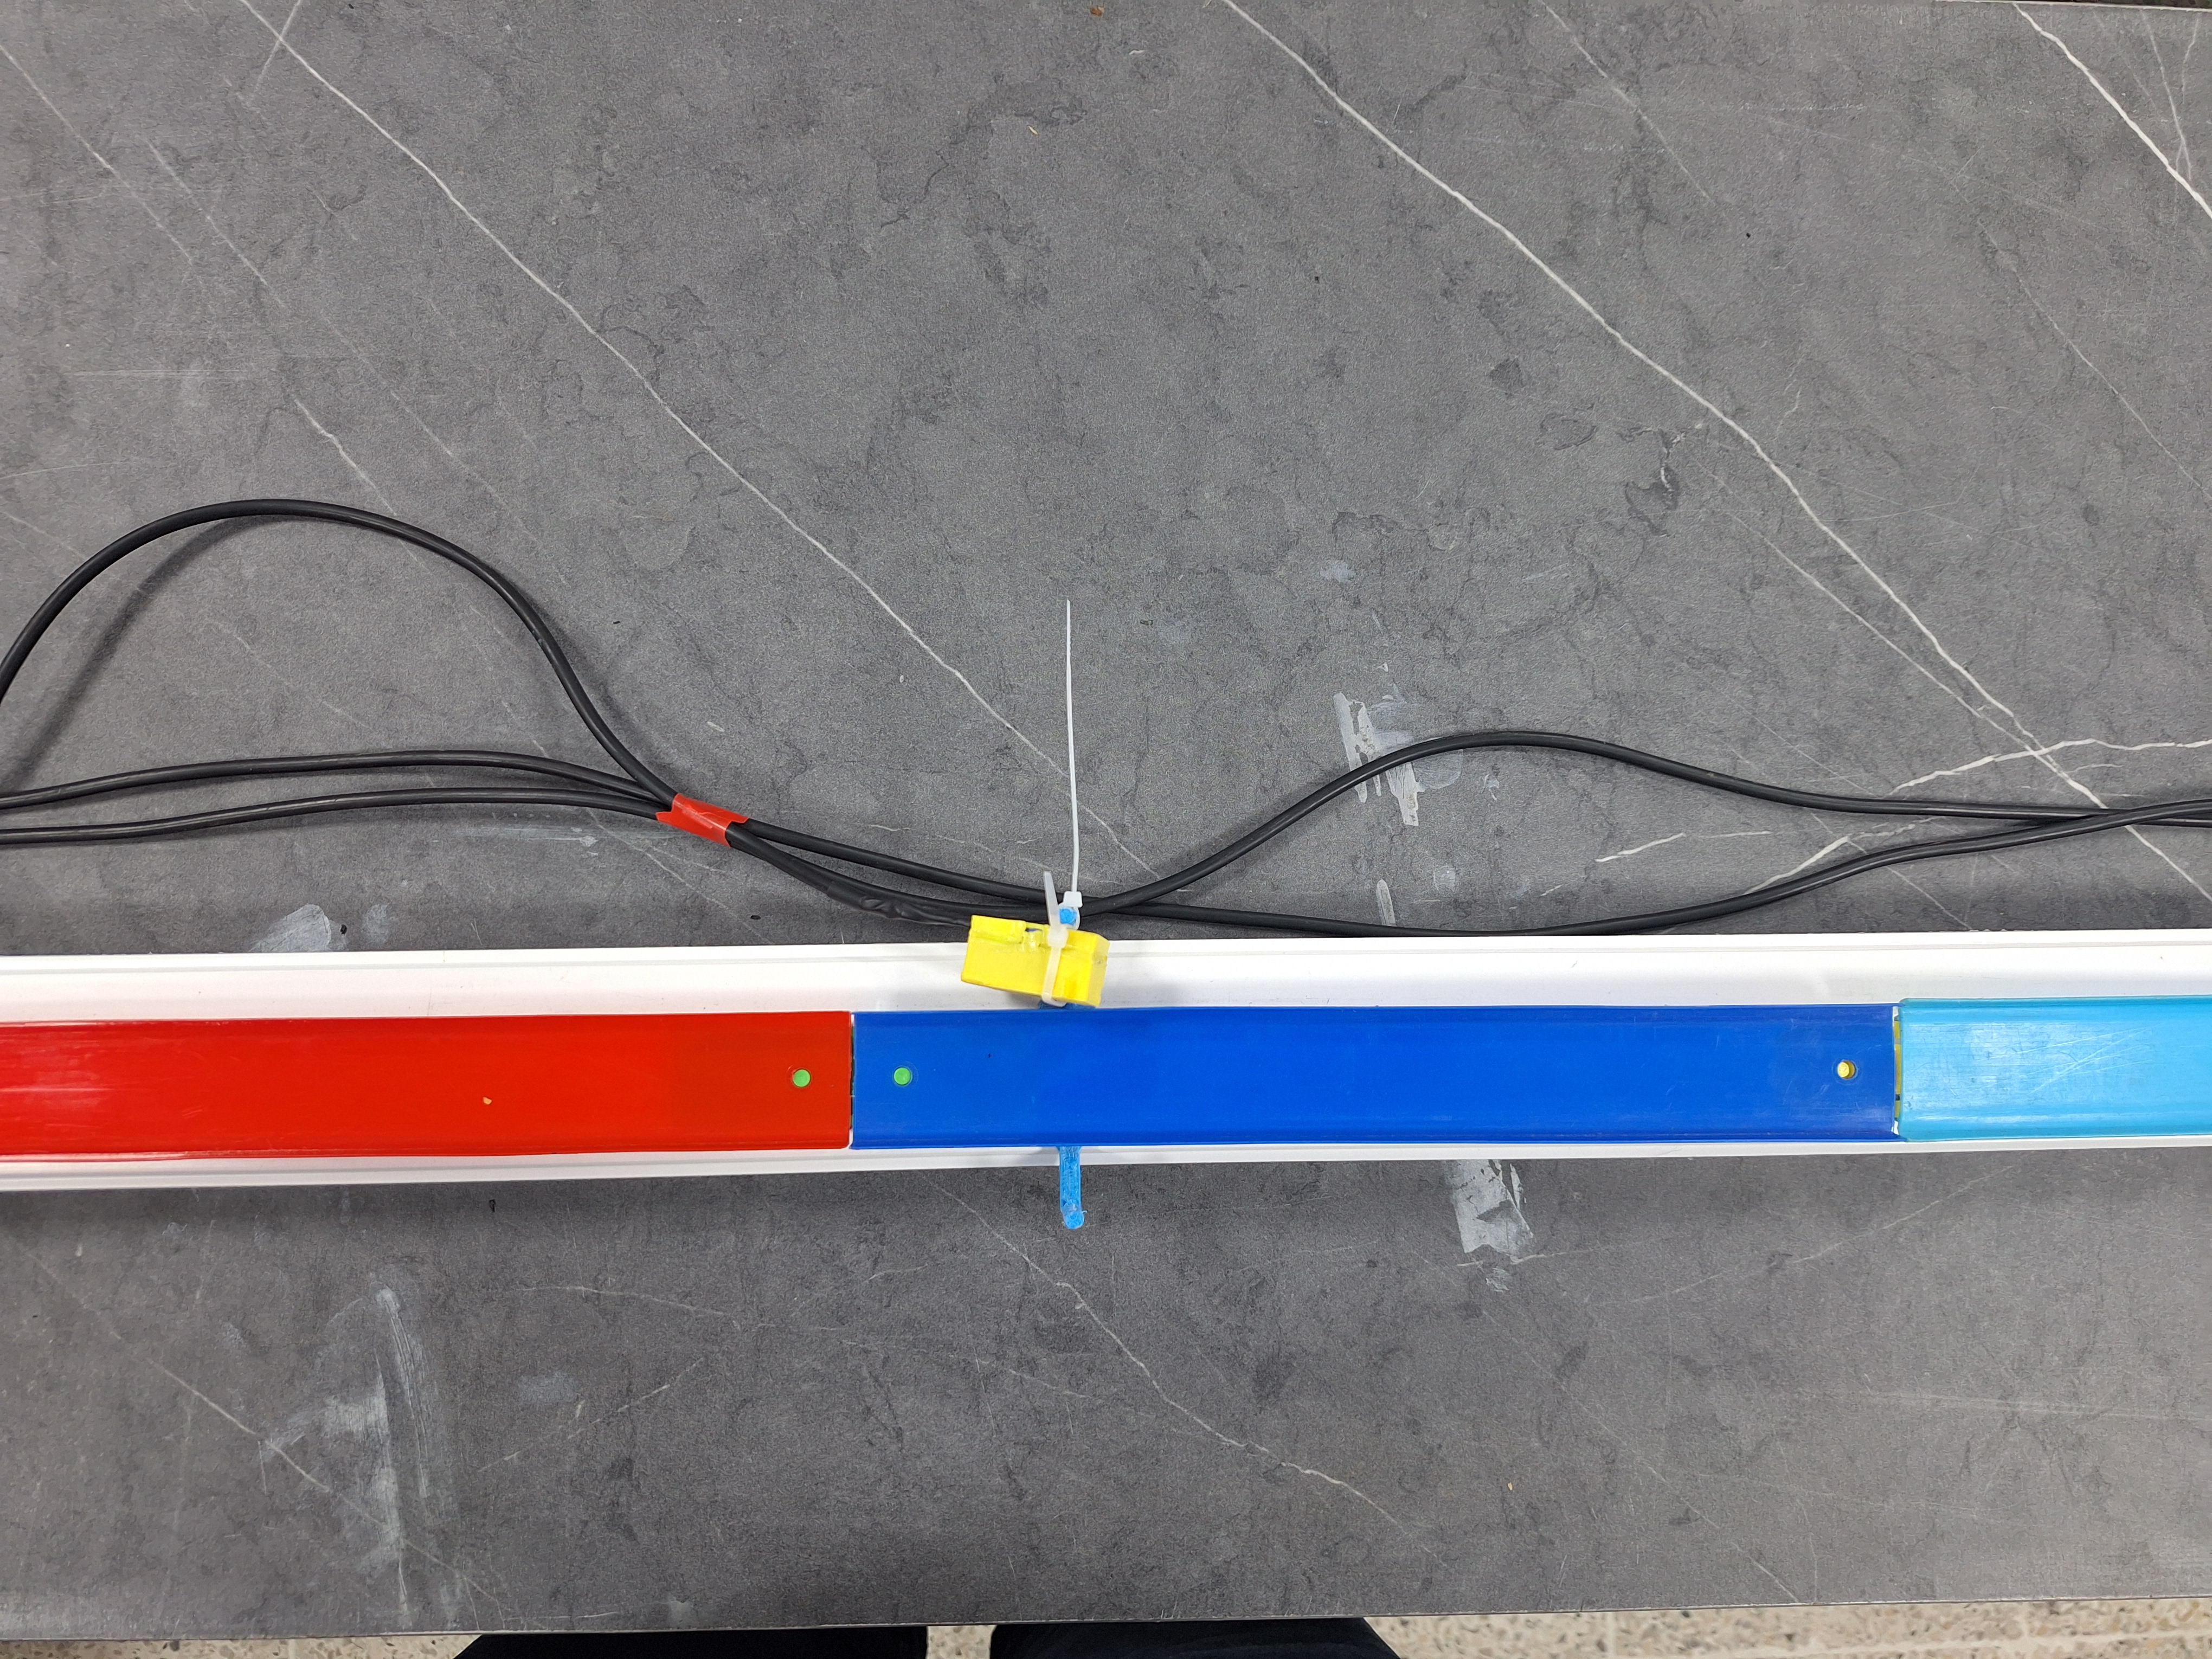
\includegraphics[width=0.45\textwidth]{figures/setup_overviewl_tramo2.jpg}}\\[0.3cm]
\subfloat[]{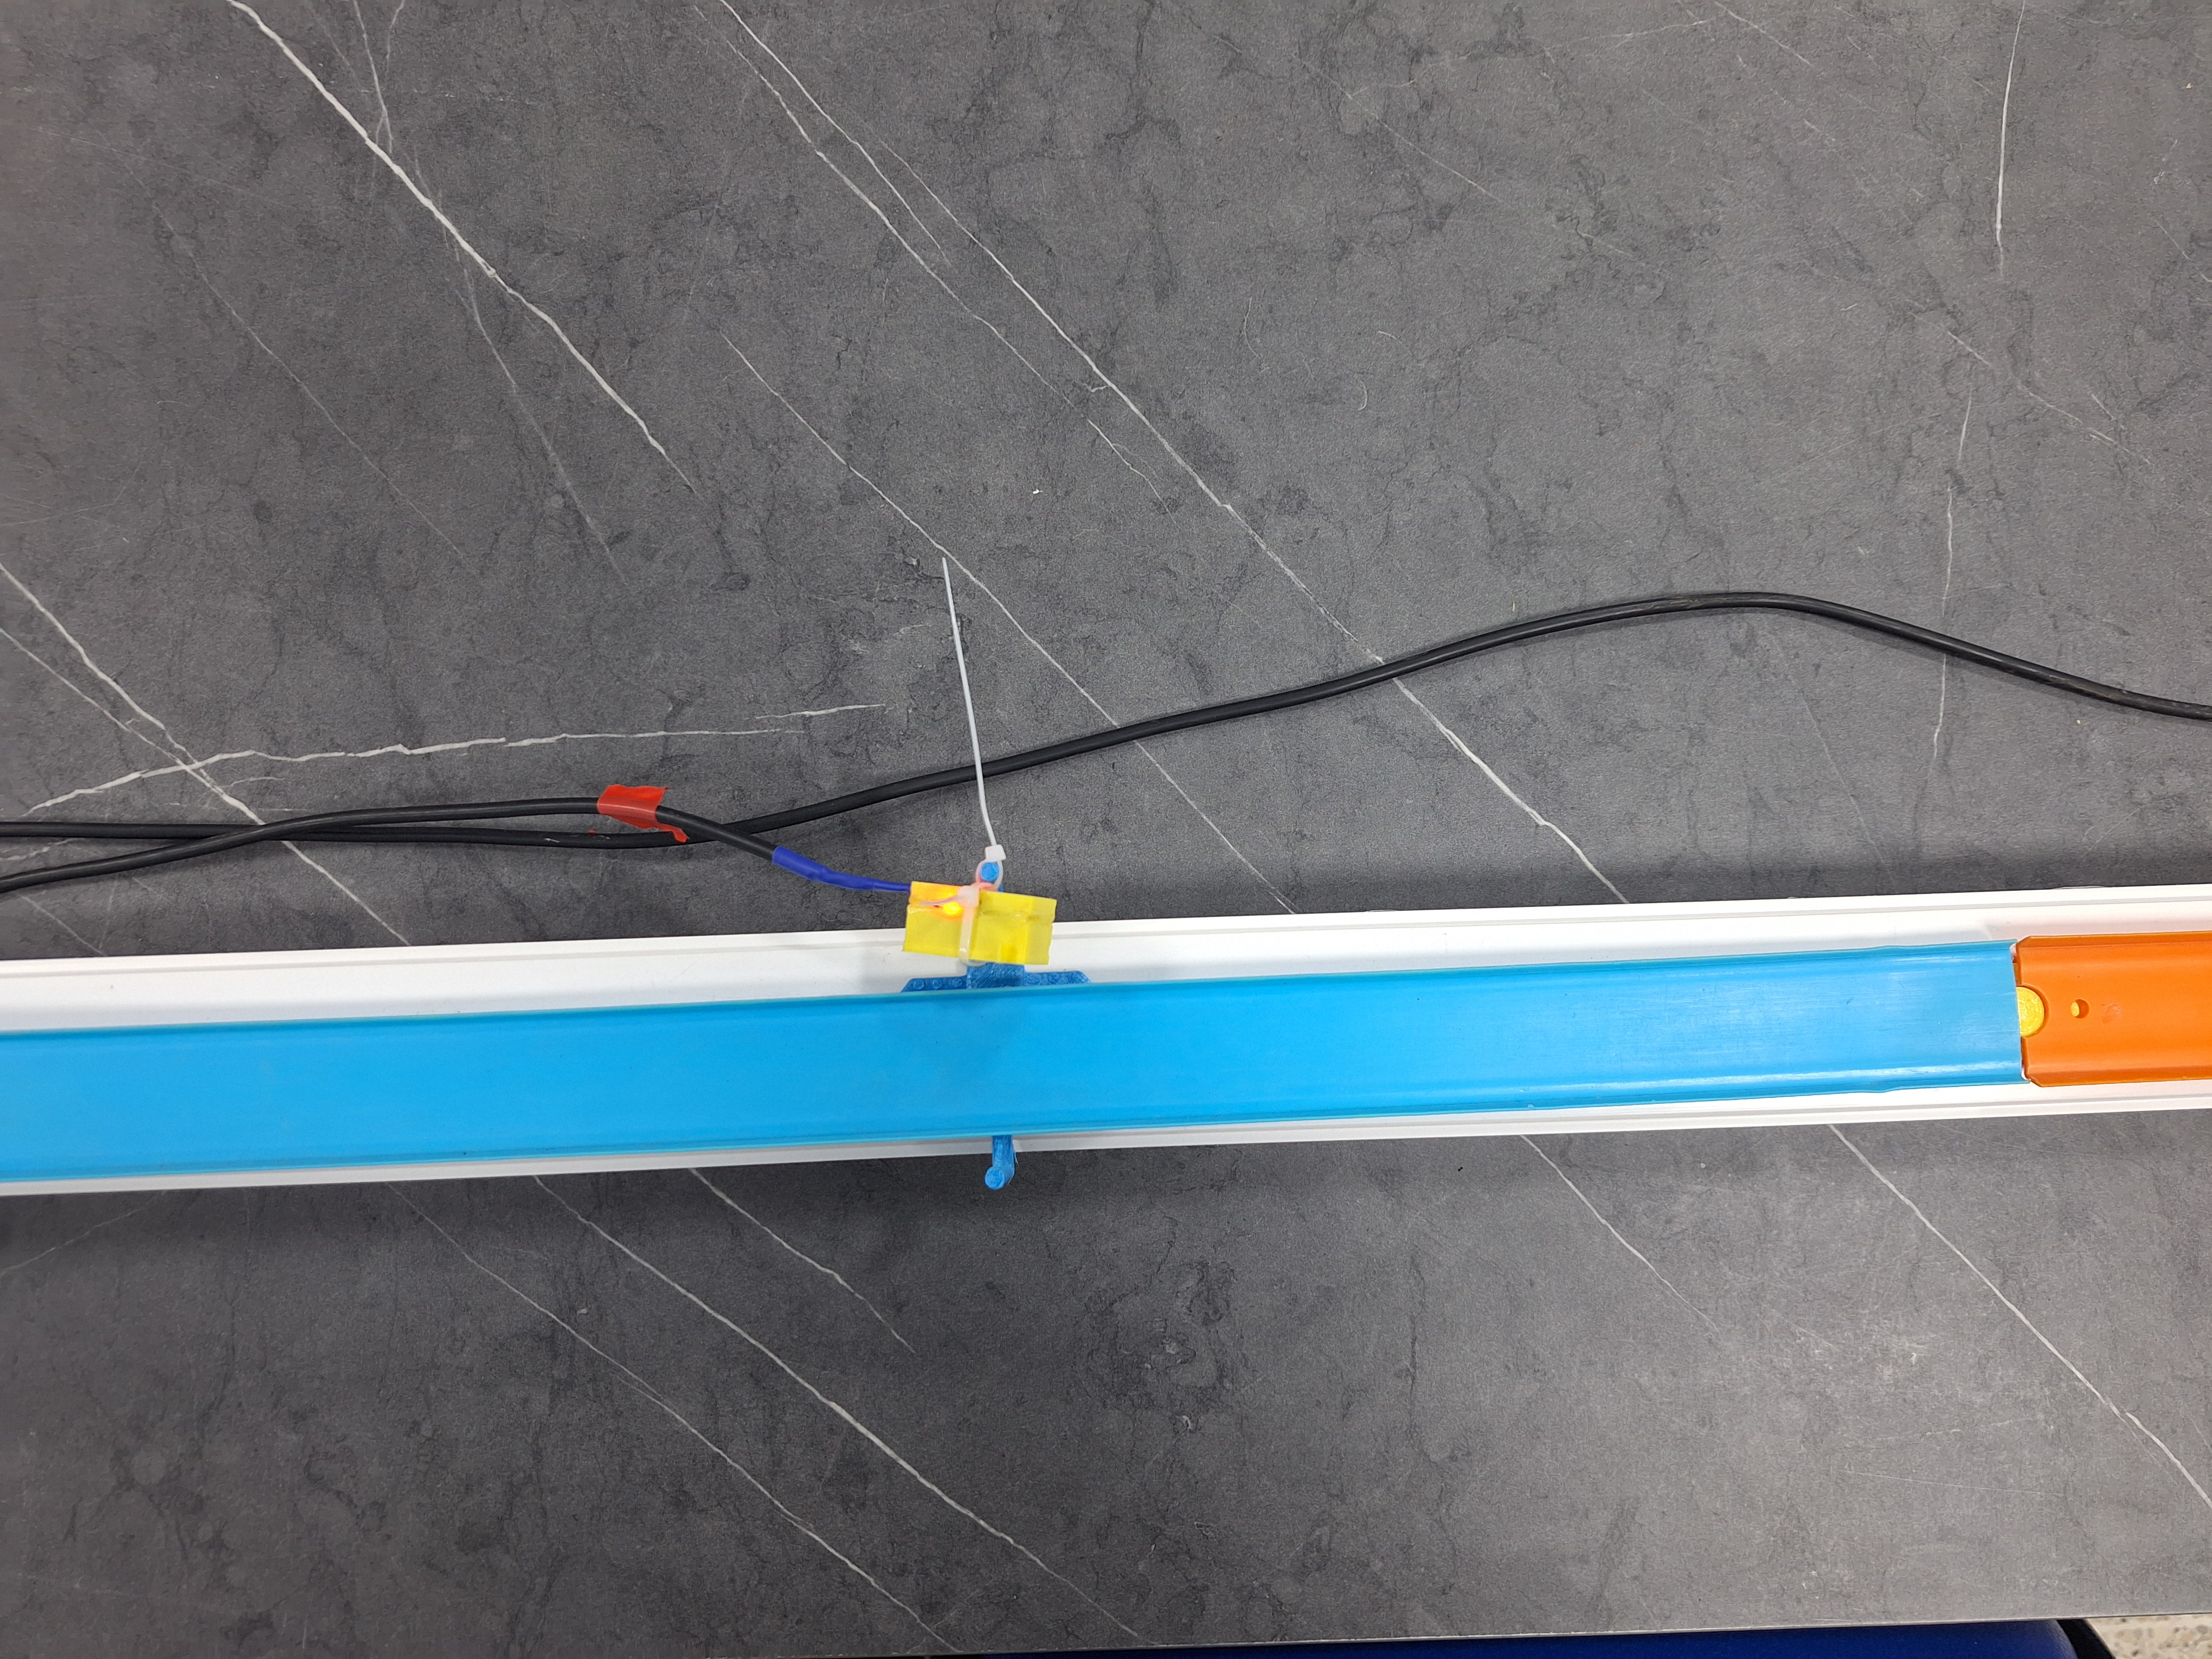
\includegraphics[width=0.45\textwidth]{figures/setup_overview_tramo3.jpg}}
\hspace{0.5cm}
\subfloat[]{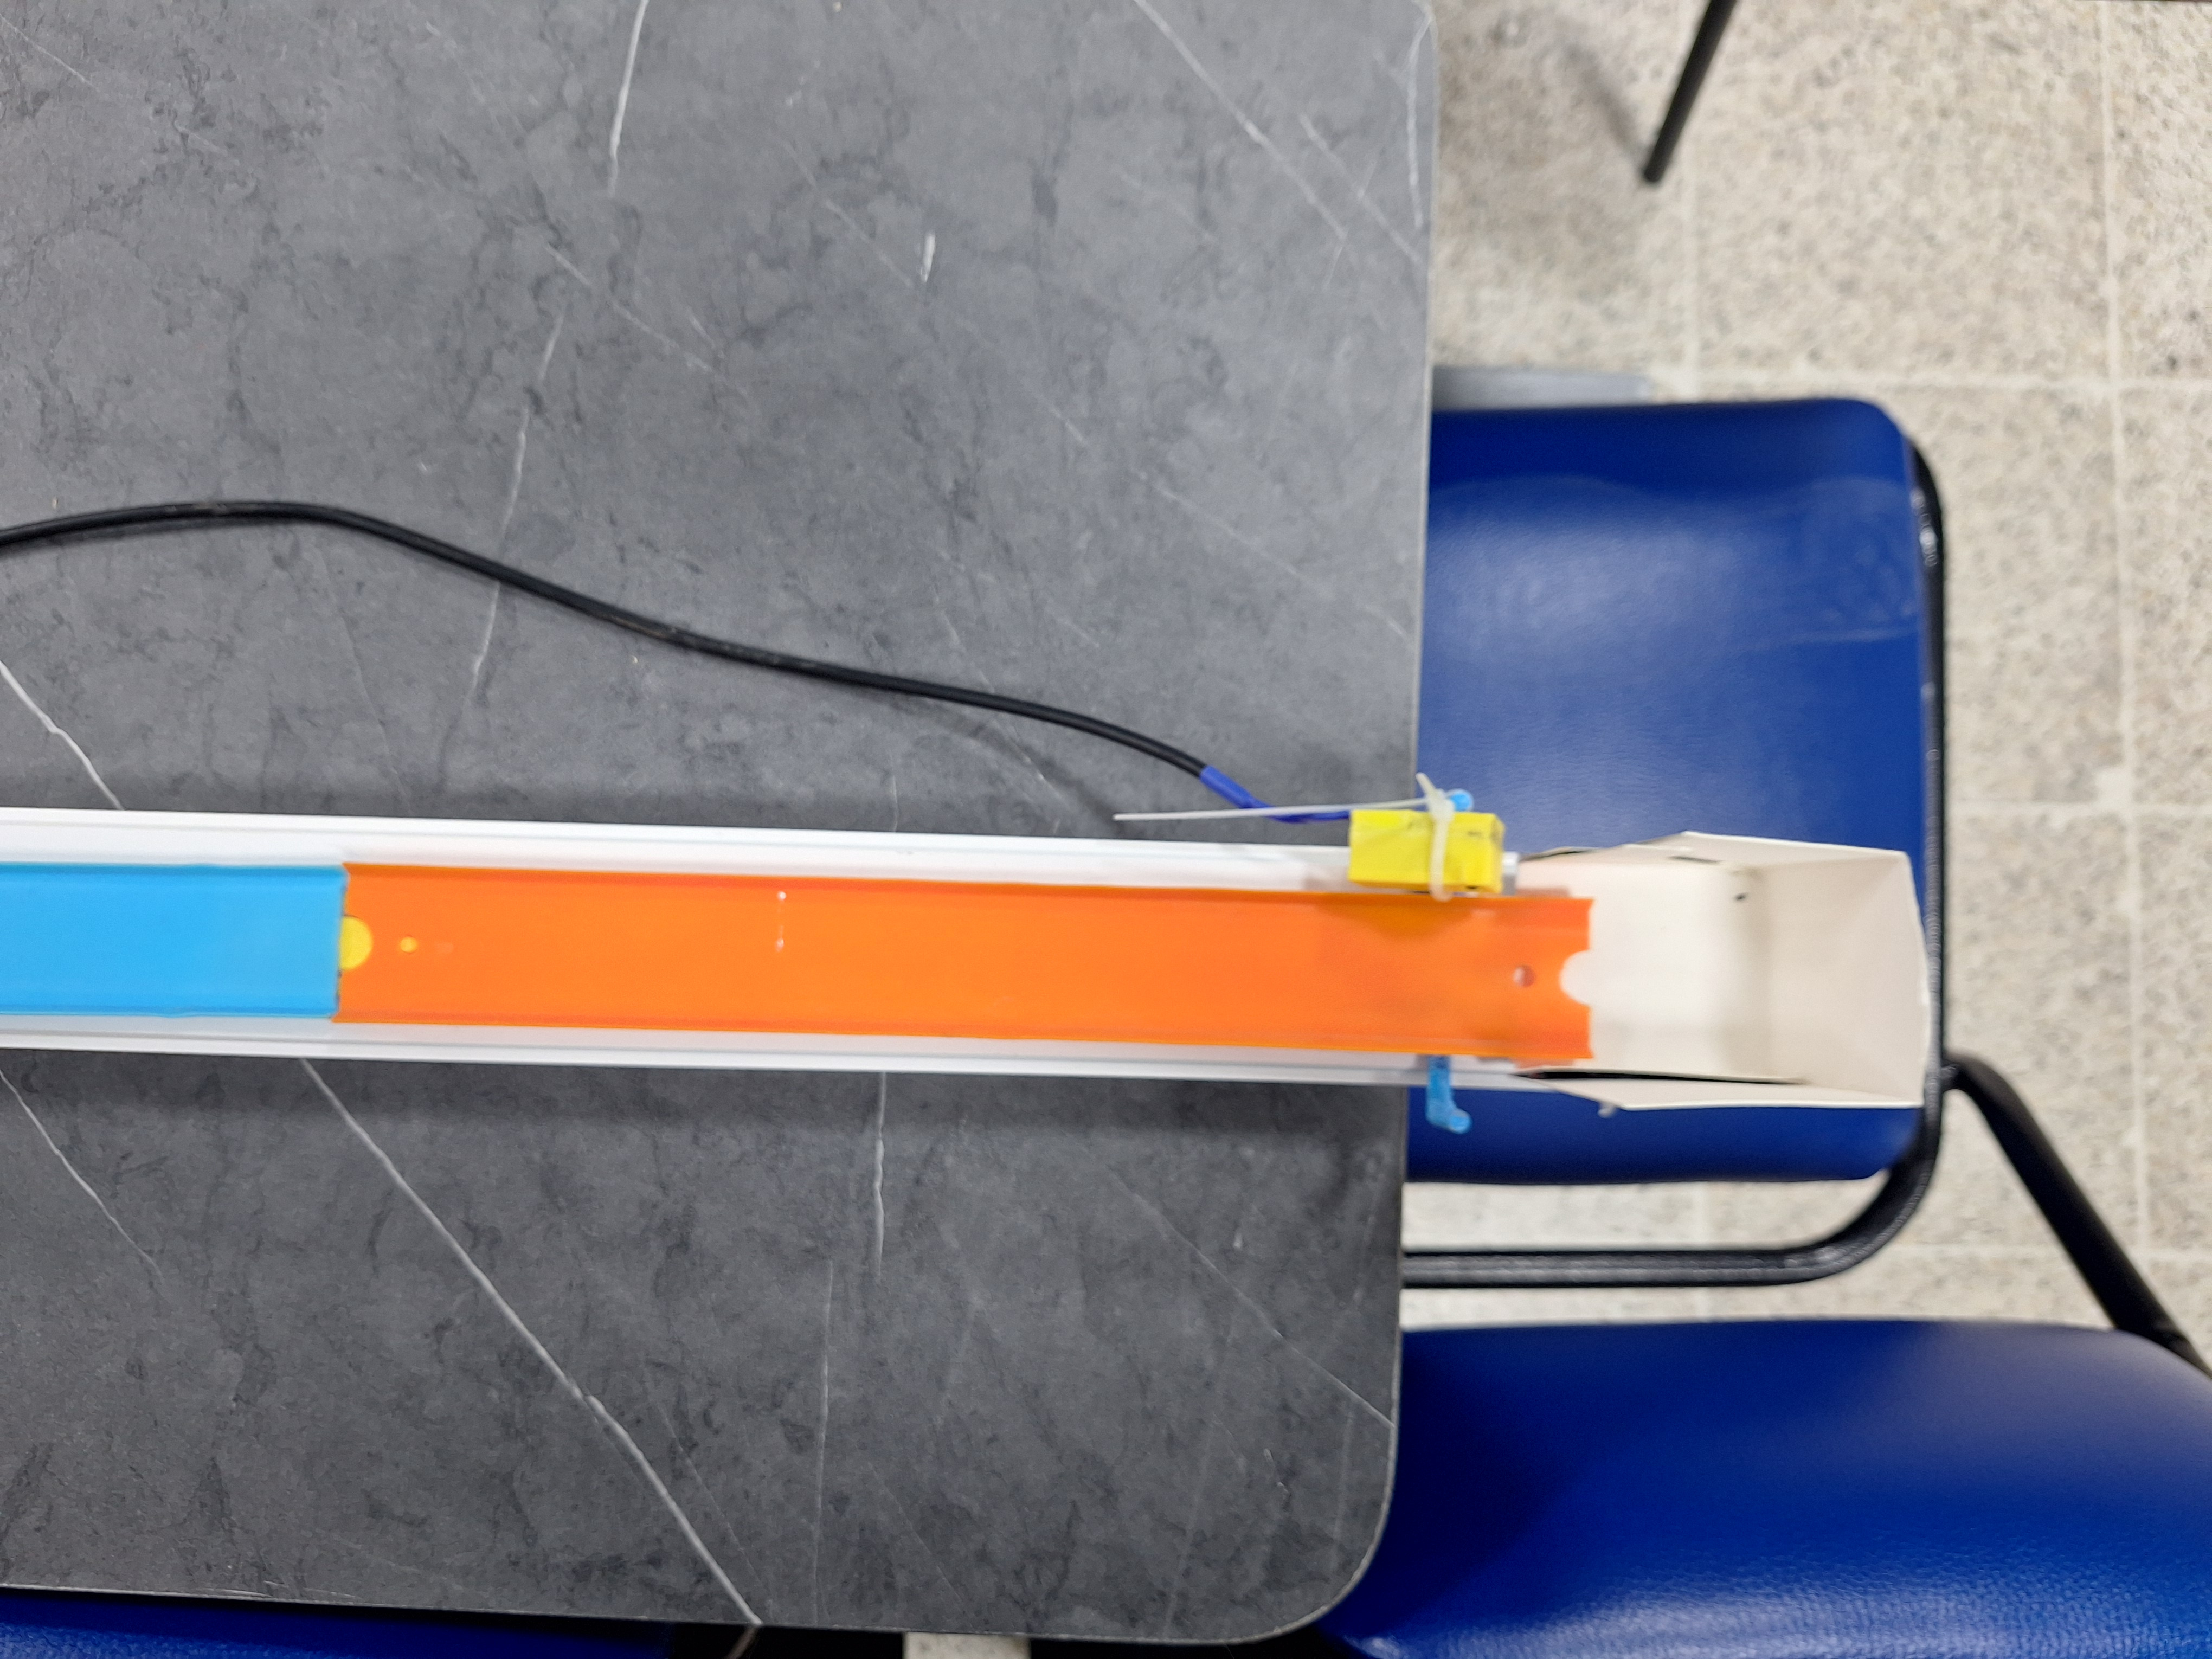
\includegraphics[width=0.45\textwidth]{figures/setup_overview_final.jpg}}
\caption{Detailed sections of the experimental setup: (a) start of the track; (b) section 2; (c) section 3; (d) arrival point and experiment completion.}
\label{fig:montaje_detalles}
\end{figure}

\begin{figure}[H]
\centering
\includegraphics[width=0.7\textwidth]{figures/setup_overview_completo.jpg}
\caption{Overall view of the IoT-based MRUA experimental setup.}
\label{fig:vista_general}
\end{figure}

To facilitate remote interaction with the experiment, a web user interface was developed to centralize system control and visualization. As shown in Figure~\ref{fig:interfaz_web}, this platform allows the user to start and stop the experimental sequence in a controlled way. In addition, the interface processes data in real time, automatically generating a plot with kinematic results after each trial. To ensure visual supervision of the process, a live video stream was integrated through a camera, allowing physical cart motion to be corroborated with received telemetry data.

\begin{figure}[H]
\centering
\includegraphics[width=0.7\textwidth]{figures/InterfazWeb.jpg}
\caption{Web interface developed for remote control and monitoring of the experiment.}
\label{fig:interfaz_web}
\end{figure}


\subsection{Sensor S1: Start of Motion}

Sensor S1 corresponds to the starting point of motion (\(t=0\)). In both modalities, this sensor acts as the experiment time trigger; therefore, the recorded time is systematically zero or very close to zero.

\begin{table}[H]
	\caption{Statistical results for Sensor S1.}
	\label{tab:s1_results}
	\centering
	\small
	\begin{tabular}{lccc}
		\toprule
		\textbf{Modality} & \textbf{\(\bar{x}\) (s)} & \textbf{\(s\) (s)} & \textbf{\(n\)} \\
		\midrule
		In-person & 0.00 & 0.00 & 35 \\
		Remote     & 0.00 & 0.00 & 35 \\
		\bottomrule
	\end{tabular}
\end{table}

\begin{figure}[H]
    \centering
    \includegraphics[width=0.7\textwidth]{figures/correlation_sensor_S1.png}
    \caption{Correlation plot for Sensor S1 (Remote vs. In-person).}
    \label{fig:corr_s1}
\end{figure}

As shown in Figure~\ref{fig:corr_s1}, data points are concentrated at the origin. The correlation coefficient is technically undefined or null (\(r \approx 0\)) because data variance is zero (\(s=0\)). This behavior is physically expected and confirms that S1 functions correctly as a synchronization reference for both manual timing and the digital control module. There are no fluctuations or experimental noise affecting this initial state.

\subsection{Sensor S2: First Intermediate Section}

Sensor S2 is located at the end of the first section of the track. Results in Table~\ref{tab:s2_results} show high consistency between mean values in both modalities (1.17 s vs 1.19 s), with comparable standard deviations (0.15 s vs 0.16 s).

\begin{table}[H]
	\caption{Statistical results for Sensor S2.}
	\label{tab:s2_results}
	\centering
	\small
	\begin{tabular}{lccc}
		\toprule
		\textbf{Modality} & \textbf{\(\bar{x}\) (s)} & \textbf{\(s\) (s)} & \textbf{\(n\)} \\
		\midrule
		In-person & 1.17 & 0.15 & 35 \\
		Remote     & 1.19 & 0.16 & 35 \\
		\bottomrule
	\end{tabular}
\end{table}

\begin{figure}[H]
    \centering
    \includegraphics[width=0.7\textwidth]{figures/correlation_sensor_S2.png}
    \caption{Correlation plot for Sensor S2 (Remote vs. In-person).}
    \label{fig:corr_s2}
\end{figure}

The plot in Figure~\ref{fig:corr_s2} shows a scattered point distribution. The calculated correlation coefficient is low (\(r < 0.3\)), classifying correlation as null or weak. This result is physically interpreted by trial independence: since "in-person trial 1" and "remote trial 1" are distinct physical events separated in time, they are subject to different random fluctuations (initial release friction, slight air-resistance variations). The lack of correlation validates that measurement error is random rather than systematic; the IoT system does not introduce bias that significantly shifts results relative to manual measurement, but instead captures natural variability of MRUA behavior.

\subsection{Sensor S3: Second Intermediate Section}

Sensor S3 captures motion at higher speed. Table~\ref{tab:s3_results} shows very similar mean times for both modalities (1.66 s vs 1.69 s), with comparable standard deviations (0.23 s vs 0.24 s), indicating consistent measurement precision in both modes.

\begin{table}[H]
	\caption{Statistical results for Sensor S3.}
	\label{tab:s3_results}
	\centering
	\small
	\begin{tabular}{lccc}
		\toprule
		\textbf{Modality} & \textbf{\(\bar{x}\) (s)} & \textbf{\(s\) (s)} & \textbf{\(n\)} \\
		\midrule
		In-person & 1.66 & 0.23 & 35 \\
		Remote     & 1.69 & 0.24 & 35 \\
		\bottomrule
	\end{tabular}
\end{table}

\begin{figure}[H]
    \centering
    \includegraphics[width=0.7\textwidth]{figures/correlation_sensor_S3.png}
    \caption{Correlation plot for Sensor S3 (Remote vs. In-person).}
    \label{fig:corr_s3}
\end{figure}

Figure~\ref{fig:corr_s3} again shows a point cloud with low correlation. The weak \(r\) value is attributed to accumulated experimental noise. As the cart travels farther, small initial acceleration variations accumulate into larger position/time deviations. The fact that both remote and in-person systems show nearly identical standard deviations (\(s=0.23\) s vs \(s=0.24\) s) demonstrates that automated detection by the control module performs comparably to manual timing, capturing natural MRUA variability with similar precision.

\subsection{Sensor S4: End of the Track}

Sensor S4 represents the final measurement point, where velocity is maximum. Results show excellent agreement between modalities, with nearly identical mean times (2.05 s vs 2.04 s) and comparable standard deviations (0.28 s vs 0.29 s).

\begin{table}[H]
	\caption{Statistical results for Sensor S4.}
	\label{tab:s4_results}
	\centering
	\small
	\begin{tabular}{lccc}
		\toprule
		\textbf{Modality} & \textbf{\(\bar{x}\) (s)} & \textbf{\(s\) (s)} & \textbf{\(n\)} \\
		\midrule
		In-person & 2.05 & 0.28 & 35 \\
		Remote     & 2.04 & 0.29 & 35 \\
		\bottomrule
	\end{tabular}
\end{table}

\begin{figure}[H]
    \centering
    \includegraphics[width=0.7\textwidth]{figures/correlation_sensor_S4.png}
    \caption{Correlation plot for Sensor S4 (Remote vs. In-person).}
    \label{fig:corr_s4}
\end{figure}

The analysis of Figure~\ref{fig:corr_s4} confirms the pattern observed in previous sensors. Both in-person and remote measurements show comparable dispersion (\(s=0.28\) s and \(s=0.29\) s, respectively), with nearly identical mean times (2.05 s vs 2.04 s). The low correlation coefficient is consistent with trial independence; each measurement captures natural variability of the MRUA phenomenon under different initial conditions. The strong agreement between modalities demonstrates that the IoT \textit{retrofitting} system successfully replicates measurement capabilities of the traditional configuration, providing reliable kinematic data for quantitative analysis of uniformly accelerated motion.

%-------------------------------------------------
% DISCUSION
%-------------------------------------------------

\section{Discussion}

\subsection{Interpretation of Temporal and Kinematic Results}

The obtained results demonstrate that the IoT \textit{retrofitting} system is capable of capturing MRUA dynamics with fidelity comparable to, and in stability even better than, the traditional in-person setup. Contrary to what is usually expected in distributed systems, remote-mode measurements showed controlled dispersion, highlighting efficient interrupt handling in the control module. Data consistency suggests that, although network latency exists, it did not degrade the quality of kinematic data collection thanks to local timestamping.

\subsection{Implications for IoT-Based Retrofitting of Physics Laboratories}

The technical feasibility of the proposed model has direct implications for modernizing educational infrastructure under limited resources. The \textit{retrofitting} approach demonstrates that classic equipment can be transformed into connected digital assets without replacing original instrumentation. The adopted modular architecture enables efficient scalability, where the sensing and control layer is decoupled from visualization and storage services. Results validate that low-cost solutions based on widely available hardware can achieve precision levels suitable for academic purposes, facilitating transition to hybrid learning environments that do not depend exclusively on physical presence in the laboratory.

\subsection{Comparison with Related Works}

When comparing results with prior literature, fundamental similarities are observed with work by Viswanadh \textit{et al.} \cite{r2} and Lustig \textit{et al.} \cite{r5} regarding the effectiveness of modular architectures for remote experiments. However, this study provides specific quantitative validation for MRUA, extending proposals by Guerrero-Osuna \textit{et al.} \cite{r4} and Fuertes \textit{et al.} \cite{r3}, which mainly focused on motor control. Unlike SmartIPL-based solutions reviewed by Zhao \cite{r6}, which depend on internal smartphone sensors, the implemented system offers fixed and dedicated infrastructure that ensures greater repeatability of test conditions while maintaining affordable deployment.

\subsection{Limitations of the Study}

Despite the satisfactory prototype performance, intrinsic limitations were identified within the study scope. First, although stability was high, the system still depends on continuous MQTT server availability for real-time data transmission. Second, the number of trials performed (n=35 per modality), while robust, is limited to a controlled university laboratory environment. In addition, the experiment operates under mechanical conditions where factors such as residual cart friction and micrometric optical sensor alignment introduce physical variations independent of IoT instrumentation.

\subsection{Future Work}

Future research lines are aimed at optimizing the perception layer and improving system robustness. Integration of higher temporal-resolution sensors and communication protocols with traffic prioritization is proposed to minimize network-latency impact. It is also pertinent to increase trial volume to strengthen statistical analysis and perform explicit latency measurements at each stage of the data chain. From a functional perspective, the system can be expanded to instrument other dynamics and energy experiments, integrating data flows with learning management systems (LMS) to automate experimental-practice assessment.

\section{Conclusions}

This study verified, under real laboratory conditions, that an IoT \textit{retrofitting} approach can modernize a classic MRUA experiment without dismantling existing infrastructure. Based on 70 independent trials (35 in-person and 35 remote), the implemented architecture with control module, infrared sensors, and web interface showed consistent behavior and technical performance comparable to the reference setup.

In performance terms, remote operation did not introduce a relevant loss of precision in the analyzed temporal variables. Instead, observed metrics indicate stability sufficient for continuous academic use, with automatic data capture that improves experiment traceability compared with exclusively manual recording. In addition, video and online visualization integration provided didactic value by facilitating the link between observed physical phenomena and recorded data.

In summary, the main contribution of this work is to show that digital transformation of physics laboratories can be addressed in a gradual, cost-effective, and replicable way. As a continuation line, it is relevant to extend validation to other mechanics setups and explicitly study the impact of network latency and periodic sensor calibration in long-term usage scenarios.

%-------------------------------------------------
% REFERENCES
%-------------------------------------------------

\reftitle{References}
\begin{thebibliography}{999}

\bibitem{r1}
Lahme, S.Z.; Klein, P.; Lehtinen, A.; M\"uller, A.; Pirinen, P.; Ron\v{c}evi\'c, L.; Su\v{s}ac, A. 
Physics lab courses under digital transformation: A trinational survey among university lab instructors about the role of new digital technologies and learning objectives. 
\textit{Phys. Rev. Phys. Educ. Res.} \textbf{2023}, \textit{19}, 020159. 
\href{https://doi.org/10.1103/PhysRevPhysEducRes.19.020159}{doi:10.1103/PhysRevPhysEducRes.19.020159}.

\bibitem{r2}
Viswanadh, K.S.; Gureja, A.; Walchatwar, N.; Agrawal, R.; Sinha, S.; 
Chaudhari, S.; Vaidhyanathan, K.; Hussain, A.M. 
Engineering End-to-End Remote Labs Using IoT-Based Retrofitting. 
\textit{IEEE Access} \textbf{2024}, \textit{PP}, 1--1. 
\href{https://doi.org/10.1109/ACCESS.2024.3523066}{doi:10.1109/ACCESS.2024.3523066}.

\bibitem{r3}
Fuertes, J.J.; Mart\'inez, J.M.; Dormido, S.; Vargas, H.; 
S\'anchez, J.; Duro, N. 
Virtual and Remote Laboratory of a DC Motor for Learning Control Theory. 
\textit{Int. J. Eng. Educ.} \textbf{2011}, \textit{27}, 1--12.

\bibitem{r4}
Guerrero-Osuna, H.A.; Garc\'ia-V\'azquez, F.A.; Ibarra-Delgado, S.; Sol\'is-S\'anchez, L.O. 
Developing a Cloud and IoT-Integrated Remote Laboratory to Enhance Education 4.0: 
An Approach for FPGA-Based Motor Control. 
\textit{Appl. Sci.} \textbf{2024}, \textit{14}, 10115.

\bibitem{r5}
Lustig, F.; Kuri\v{s}\v{c}\'ak, P.; Brom, P.; Dvo\v{r}\'ak, J. 
Open Modular Hardware and Software Kit for Creations of Remote Experiments Accessible from PC and Mobile Devices. 
\textit{Int. J. Online Eng. (iJOE)} \textbf{2016}, \textit{12}, 30--36. 
\href{https://doi.org/10.3991/ijoe.v12i07.5833}{doi:10.3991/ijoe.v12i07.5833}.

\bibitem{r6}
Zhao, Y. 
Smartphone-Based Undergraduate Physics Labs: A Comprehensive Review. 
\textit{IEEE Access} \textbf{2024}, \textit{13}, 1106--1132. 
\href{https://doi.org/10.1109/ACCESS.2024.3523066}{doi:10.1109/ACCESS.2024.3523066}.

\bibitem{r7}
Dizdarevic, J.; Jukan, A.
Engineering an IoT--Edge--Cloud Computing System Architecture: Lessons Learnt from an Undergraduate Laboratory Course.
\textit{IoT} \textbf{2022}, \textit{3}, 145--163.
\href{https://doi.org/10.3390/iot3010010}{doi:10.3390/iot3010010}.

\bibitem{r8}
Azad, A.K.M.
Use of Internet of Things for Remote Laboratory Settings.
\textit{IoT} \textbf{2021}, \textit{2}, 203--232.
\href{https://doi.org/10.3390/iot2020011}{doi:10.3390/iot2020011}.

\bibitem{r9}
Palmer, C.; Roullier, B.; Aamir, M.; McQuade, F.; Stella, L.; Anjum, A.
Digital Twinning Remote Laboratories for Online Practical Learning.
\textit{Sensors} \textbf{2022}, \textit{22}, 2351.
\href{https://doi.org/10.3390/s22062351}{doi:10.3390/s22062351}.

\bibitem{r10}
Atzori, L.; Iera, A.; Morabito, G. 
The Internet of Things: A survey. 
\textit{Comput. Netw.} \textbf{2010}, \textit{54}, 2787--2805. 
\href{https://doi.org/10.1016/j.comnet.2010.05.010}{doi:10.1016/j.comnet.2010.05.010}.

\bibitem{r11}
Hevner, A.R.; March, S.T.; Park, J.; Ram, S. 
Design Science in Information Systems Research. 
\textit{MIS Q.} \textbf{2004}, \textit{28}, 75--105.

\bibitem{r12}
ISO/IEC. 
\textit{ISO/IEC 15288:2015 Systems and Software Engineering—System Life Cycle Processes}; 
International Organization for Standardization: Geneva, Switzerland, 2015.

\bibitem{r13}
Mattel, Inc.
\textit{Hot Wheels Track Sets}.
Available online: \url{https://shop.mattel.com/pages/hot-wheels} (accessed on 5 December 2025).

\bibitem{r14}
Mattel, Inc.
\textit{Hot Wheels Cars}.
Available online: \url{https://shop.mattel.com/collections/hot-wheels-cars} (accessed on 5 December 2025).

\bibitem{r15}
Vishay Intertechnology, Inc.
\textit{TCRT5000 Reflective Optical Sensor}.
Available online: \url{https://www.vishay.com/docs/83751/tcrt5000.pdf} (accessed on 5 December 2025).

\bibitem{r16}
Espressif Systems.
\textit{ESP32-WROOM-32 Datasheet}.
Available online: \url{https://www.espressif.com/sites/default/files/documentation/esp32-wroom-32_datasheet_en.pdf} (accessed on 5 December 2025).

\bibitem{r17}
Thingiverse.
\textit{Mechanical Support for Track-Based Experiments (Thing 3630616)}.
Available online: \url{https://www.thingiverse.com/thing:3630616}
(accessed on 5 December 2025).

\bibitem{r18}
Thingiverse.
\textit{3D Printed Modular Track Components (Thing 3485484)}.
Available online: \url{https://www.thingiverse.com/thing:3485484}
(accessed on 5 December 2025).

\bibitem{r19}
Thingiverse.
\textit{3D Printed Structural Reinforcement Parts (Thing 4381935)}.
Available online: \url{https://www.thingiverse.com/thing:4381935}
(accessed on 5 December 2025).

\bibitem{r20}
Thingiverse.
\textit{3D Printed Mechanical Pusher Mechanism (Thing 2806324)}.
Available online: \url{https://www.thingiverse.com/thing:2806324}
(accessed on 5 December 2025).

\bibitem{r21}
Tower Pro.
\textit{SG90 Micro Servo Motor Datasheet}.
Available online: \url{http://www.ee.ic.ac.uk/pjs99/projects/servo/sg90_datasheet.pdf} (accessed on 5 December 2025).

\bibitem{r22}
StepperOnline.
\textit{NEMA 17 Stepper Motor Bipolar Datasheet}.
Available online: \url{https://www.omc-stepperonline.com/download/17HS19-2004S1.pdf} (accessed on 5 December 2025).

\bibitem{r23}
STMicroelectronics.
\textit{L298N Dual H-Bridge Motor Driver Datasheet}.
Available online: \url{https://www.st.com/resource/en/datasheet/l298.pdf} (accessed on 5 December 2025).

\bibitem{r24}
Generic Electronics Suppliers.
\textit{LCD 20x4 Display with I\textsuperscript{2}C Interface Datasheet}.
Available online: \url{https://www.sparkfun.com/datasheets/LCD/HD44780.pdf} (accessed on 5 December 2025).

\bibitem{r25}
Generic Electronics Suppliers.
\textit{Tactile Push Button Switch for Breadboard}.
Available online: \url{https://www.adafruit.com/product/367} (accessed on 5 December 2025).

\bibitem{r26}
USB Implementers Forum.
\textit{USB Type-C Cable Specification}.
Available online: \url{https://www.usb.org/sites/default/files/USB%20Type-C%20Spec%20R2.0%20-%20August%202019.pdf} (accessed on 5 December 2025).

\bibitem{r27}
IEEE.
\textit{IEEE Standard for Wireless LAN Medium Access Control (MAC) and Physical Layer (PHY) Specifications}.
Available online: \url{https://ieeexplore.ieee.org/document/9363693} (accessed on 5 December 2025).

\bibitem{r28}
Generic Electronics Suppliers.
\textit{Dupont Jumper Wires (Male-Female and Female-Female)}.
Available online: \url{https://www.adafruit.com/category/289} (accessed on 5 December 2025).

\bibitem{r29}
Generic Electronics Suppliers.
\textit{Plastic Project Enclosure Box (135x75x40 mm)}.
Available online: \url{https://www.digikey.com/en/products/filter/enclosures/287} (accessed on 5 December 2025).

\bibitem{r30}
Generic Electronics Suppliers.
\textit{AC-DC Power Adapter 12V/1A}.
Available online: \url{https://www.digikey.com/en/products/filter/power-supplies-external-internal-off-board/171} (accessed on 5 December 2025).

\bibitem{r31}
Insta360.
\textit{Insta360 Link---4K AI Webcam Technical Specifications}.
Available online: \url{https://onlinemanual.insta360.com/link/en-us/introduction} (accessed on 5 December 2025).

\bibitem{r32}
Raspberry Pi Ltd.
\textit{Raspberry Pi 4 Model B Product Brief}.
Available online: \url{https://datasheets.raspberrypi.com/rpi4/raspberry-pi-4-product-brief.pdf} (accessed on 5 December 2025).

\bibitem{r33}
EMQ Technologies Co., Ltd.
\textit{EMQX---MQTT Platform for IoT Data Streaming Documentation}.
Available online: \url{https://docs.emqx.com/en/emqx/v5.0/} (accessed on 5 December 2025).

\bibitem{r34}
EMQ Technologies Co., Ltd.
\textit{MQTTX: Your All-in-One MQTT Client Toolbox Documentation}.
Available online: \url{https://mqttx.app/docs} (accessed on 5 December 2025).

\bibitem{r35}
OpenJS Foundation.
\textit{Node.js API Documentation}.
Available online: \url{https://nodejs.org/api/} (accessed on 5 December 2025).

\bibitem{r36}
OpenJS Foundation.
\textit{Express API Reference}.
Available online: \url{https://expressjs.com/en/4x/api.html} (accessed on 5 December 2025).

\bibitem{r37}
MongoDB, Inc.
\textit{MongoDB Documentation}.
Available online: \url{https://www.mongodb.com/docs/manual/} (accessed on 5 December 2025).

\bibitem{r38}
Mongoose.
\textit{Mongoose ODM API Documentation}.
Available online: \url{https://mongoosejs.com/docs/api.html} (accessed on 5 December 2025).

\bibitem{r39}
Vercel, Inc.
\textit{Next.js Documentation}.
Available online: \url{https://nextjs.org/docs} (accessed on 5 December 2025).

\bibitem{r40}
Meta Platforms, Inc.
\textit{React Reference Documentation}.
Available online: \url{https://react.dev/reference/react} (accessed on 5 December 2025).

\bibitem{r41}
Arduino AG.
\textit{Arduino IDE 2.x Documentation}.
Available online: \url{https://www.arduino.cc/en/software} (accessed on 5 December 2025).

\bibitem{r42}
Python Software Foundation.
\textit{Python 3 Documentation}.
Available online: \url{https://docs.python.org/3/} (accessed on 5 December 2025).

\bibitem{r43}
Eraser Labs, Inc.
\textit{Eraser---AI Co-Pilot for Technical Design and Documentation}.
Available online: \url{https://www.eraser.io} (accessed on 5 December 2025).

\bibitem{r44}
OpenAI. \textit{ChatGPT}.
Available online: \url{https://chat.openai.com} (accessed on 23 January 2026). Content generated with the assistance of ChatGPT.

\bibitem{r45}
Santiago Sosa Mej\'ia.
\textit{RemotePhysicsLab: Prototipo de laboratorio de f\'isica h\'ibrido basado en IoT}. 
Repositorio GitHub. 
Available online: \url{https://github.com/waltersosa/RemotePhysicsLab.git} (accessed on 5 December 2025).

\end{thebibliography}

\end{document}